% sage_latex_guidelines.tex V1.20, 14 January 2017

\documentclass[Review,sagev,times]{sagej}

\usepackage{amsmath}
\usepackage{booktabs}
\usepackage[makeroom]{cancel}
\usepackage{changes}
\usepackage{subcaption}
\usepackage{tabularx}
\usepackage{moreverb,url}
\usepackage[colorlinks,bookmarksopen,bookmarksnumbered,citecolor=red,urlcolor=red]{hyperref}

\newcommand\BibTeX{{\rmfamily B\kern-.05em \textsc{i\kern-.025em b}\kern-.08em
T\kern-.1667em\lower.7ex\hbox{E}\kern-.125emX}}

\def\volumeyear{2019}

\begin{document}

\runninghead{Di Stasio et al.}

\title{Effect of the proximity to the $\mathbf{0^{\circ}/90^{\circ}}$ interface on Energy Release Rate of fiber/matrix interface crack growth in the  $\mathbf{90^{\circ}}$-ply of a cross-ply laminate under tensile loading}

\author{Luca Di Stasio\affilnum{1,2}, Janis Varna\affilnum{1} and Zoubir Ayadi\affilnum{2}}

\affiliation{
\affilnum{1}Lule\aa\ University of Technology, University Campus, SE-97187 Lule\aa, Sweden\\
\affilnum{2}Universit\'e de Lorraine, EEIGM, IJL, 6 Rue Bastien Lepage, F-54010 Nancy, France
}

\corrauth{Luca Di Stasio\\
Lule\aa\ University of Technology\\
University Campus\\
SE-97187 Lule\aa, Sweden}

\email{luca.di.stasio@ltu.se}

\begin{abstract}
Models of Representative Volume Elements (RVEs) of cross-ply laminates with different geometric configurations and damage states are studied. Debond growth is characterized by the estimation of the Mode I and Mode II Energy Release Rate (ERR) using the Virtual Crack Closure Technique (VCCT). It is found that the presence of the $0^{\circ}/90^{\circ}$ interface and the thickness of the $0^{\circ}$ layer have no effect, apart from laminates with \emph{ultra-thin} $90^{\circ}$ plies where it is however modest. The present analysis support the claim that debond growth is not affected by the ply-thickness effect.
\end{abstract}

\keywords{Polymer-matrix Composites (PMCs), Fibre/matrix bond, Debonding, Finite Element Analysis (FEA)}

\maketitle

%%%%%%%%%%%%%%%%%%%%%%%%%%%%%%%%%%%%%%%%%%%%%%%%%%%%%%%%%%%%%%%%%%%
% 1. INTRODUCTION
%%%%%%%%%%%%%%%%%%%%%%%%%%%%%%%%%%%%%%%%%%%%%%%%%%%%%%%%%%%%%%%%%%%

\section{Introduction}

Since the development of the \emph{spread tow} technology or ``FUKUI method''~\cite{Kawabe2008}, significant efforts have been directed toward the characterization of \emph{thin-ply} laminates~\cite{Yamaguchi2005,Sihn2007,Yokozeki2008,Yokozeki2010,Saito2012,Arteiro2013,Arteiro2014,Amacher2014,Guillamet2014,Cugnoni2018} and their application to mission-critical structures in the aerospace sector~\cite{Kopp2017}.\\%~\cite{Moon2011,Kim2017,Kopp2017,McCarville2018}.\\
At the lamina level, the use of \emph{thin-plies} leads to more regular and homogeneous microstructures~\cite{Saito2012,Amacher2014}. Measurements of ply level properties (tensile and compressive modulus, Poisson's ratio, ultimate tensile strength,tensile onset of damage, interlaminar shear strength) on Uni-Directional (UD) specimens ($\left[0_{m}^{\circ}\right]$ and $\left[90_{m}^{\circ}\right]$) revealed no remarkable difference with average properties available in the literature for the same type of fiber, nor showed any particular dependence on the ply thickness~\cite{Amacher2014}. Only an increase of the ultimate compressive strength in the fiber direction was observed with very thin plies ($\sim4$ fiber diameters), although with very scattered values. The authors claim the increase to be due to the fiber arrangement's increased regularity which prevents the onset of fiber microbuckling~\cite{Amacher2014}. A number of researchers~\cite{Yamaguchi2005,Sihn2007,Yokozeki2008} has reported improvements in fatigue life with the use of \emph{thin-plies}, which are explained as a consequence of delayed propagation of free edge delaminations and intralaminar cracks. Several researchers have analyzed the effect of \emph{thin-plies} on damage development under static~\cite{Sihn2007,Yokozeki2008,Yokozeki2010,Saito2012,Arteiro2013,Arteiro2014,Amacher2014}, fatigue~\cite{Yamaguchi2005,Sihn2007,Yokozeki2008,Yokozeki2010,Amacher2014} and impact loadings~\cite{Sihn2007,Yokozeki2008,Yokozeki2010,Amacher2014}. It seems apparent that \emph{thin-ply} laminates possess an increased ability to delay, and in some cases even suppress, the onset and propagation of intralaminar cracks (called often transverse or matrix or micro-cracks).\\
The first stage in the appearance of transverse cracks is known to be the occurrence of fiber/matrix interface cracks (also referred to as debonds), which grow along the fiber arc direction, then kink out of the interface and coalesce forming a transverse crack~\cite{Bailey1981}. Different approaches have been applied to model the initiation and growth of debonds~\cite{Krueger2013}. The Cohesive Zone Model (CZM) has been used to mimic the propagation of debonds along fiber interfaces; coupled with a failure criterion for the matrix, it has provided simulations of the growth of transverse cracks starting from a virgin material~\cite{Kushch2011,Canal2012,Bouhala2013,Herraez2015}. The strength of the CZM, and its main requirement for a correct implemetation, lies in the elimination of the stress and displacement singularity that exists at the crack tip in the Linear Elastic Fracture Mechanics (LEFM) solution, as the crack tip is not explicitly modeled and the failure process is ``smeared'' over the finite length of the cohesive element. The main advantages of this approach are the possibility to observe the development of a simulated crack path and to record a load-displacement curve to be compared with experimental measurements. The fracture toughness (or critical Energy Release Rate) dependence on mode-mixity in the case of the interface crack~\cite{Mantic2009} was successfully incorporated in a cohesive zone model by Freed and Banks-Sills~\cite{Freed2008}. However, different problems were reported~\cite{Jin2005} on the use of cohesive elements to simulate a bimaterial interface crack. It was observed that, for mixed-mode fracture in general, a single cohesive zone length might not simultaneously cancel both the tensile and shear stress singularity at the crack tip and thus fail to satisfy the fundamental requirement of the CZM approach. Also, it was concluded that energy dissipation at the cohesive zone tip could be neglected only with high enough values of the initial tensile and shear stiffnesses. A further issue which arises in the use of cohesive elements is the selection of appropriate values for the material parameters required by the model (critical stress and Energy Release Rate). Two options are available: adopting values measured from macroscopic tests (e.g. Double Cantilever Beam) or calibrating the parameters through inverse estimation by approximation of the macroscopic stress-strain response of the specific specimen the RVE modeled is representing. Finally, the failure mechanisms proposed by the Cohesive Zone Model might not represent the actual physics of the fiber/matrix interface failure process. It was shown~\cite{Asp1995} that the triaxiality of the matrix stress state in the inter-fiber region may be the driver of brittle matrix failure at or very close to the interface through a cavitation-like mechanism~\cite{Pawlak2014}. It thus seems likely that brittle failure at the interface may create an initial flaw from which debonding occurs in a fast and unstable manner, that could be modeled by the classic Griffith's criterion of LEFM. Linear Elastic Fracture Mechanics obviates many of the drawbacks highlighted for Cohesive Zone Modeling. The analysis focuses on the evaluation of Mode I and Mode II Energy Release Rate (ERR) at the crack tip by means of the Virtual Crack Closure Technique (VCCT)~\cite{Krueger2004} or the J-Integral method~\cite{Rice1968}. The stress and strain fields, required for the ERR computation, can be solved by application of different methodologies such as analytical solutions~\cite{Toya1974}, the Boundary Element Method (BEM)~\cite{Paris1996} or the Finite Element Method (FEM)~\cite{Zhuang2018}. This approach presents nonetheless some limitations: it describes propagation of the debond and not its initiation; the role of friction in the contact zone is still an open issue; consensus is still lacking on a proper criterion for crack propagation in mixed mode. Finite fracture mechanics~\cite{MunozReja2016} is one way to address the initiation problem. Different studies have followed the LEFM approach and analyzed models of one or two fibers in an effectively infinite matrix~\cite{Correa2011,Correa2013,Correa2014,Sandino2016,Sandino2018} and of an hexagonal cluster of fibers in an effectively infinite homogenized UD composite~\cite{Varna2017,Zhuang2018}. The problem of debond growth along the fiber-matrix interface in a cross-ply laminate has been only treated very recently in~\cite{Velasco2018,Paris2018}, where authors embed a single partially debonded fiber in an effectively infinite homogenized $90^{\circ}$ ply bounded by homogenized $0^{\circ}$ layers. Thus, the effect of debond-debond interaction and of the relative proximity of a $0^{\circ}/90^{\circ}$ interface on debond ERR in cross-ply laminates is yet to be addressed. The present work is devoted to this problem. Our interest however is not to investigate the sequence of failure events, which would require knowledge of appropriate failure criteria and properties, but rather to understand which parameters may make debond growth energetically favorable and which may prevent it. Models of Repeating Unit Cells (RUCs) are developed to represent laminates with different degrees of damage in the $90^{\circ}$ ply (here only in the form of debonds). The number of fully bonded fibers across the thickness of the $90^{\circ}$ ply is varied in order to investigate the effect of the proximity of the $0^{\circ}/90^{\circ}$ interface. The thickness of the bounding $0^{\circ}$ layers is also used as a parameter of the study. The stress and strain fields are solved with the Finite Element Method in Abaqus~\cite{abq12} and the debond (crack) is characterized by its Mode I and Mode II ERR calculated with the VCCT.

%%%%%%%%%%%%%%%%%%%%%%%%%%%%%%%%%%%%%%%%%%%%%%%%%%%%%%%%%%%%%%%%%%%
% 2. RVE MODELS AND FE DISCRETIZATION
%%%%%%%%%%%%%%%%%%%%%%%%%%%%%%%%%%%%%%%%%%%%%%%%%%%%%%%%%%%%%%%%%%%

\section{RVE models \& FE discretization}

% 2.1 Introduction and nomenclature

\subsection{Introduction \& nomenclature}\label{subsec:names}

In the present work, we investigate debond development under in-plane longitudinal tension in $\left[0_{m\cdot k\cdot2L}^{\circ},90_{k\cdot2L}^{\circ},0_{m\cdot k\cdot2L}^{\circ}\right]$ laminates. The interaction between debonds in the presence of an interface with a stiff layer is studied with the use of different Repeating Unit Cells (RUCs)  (see Figures~\ref{fig:laminateModelsA} and~\ref{fig:laminateModelsB}), in which only the central fiber is partially debonded. Repetition of the composite RUC occurs along the in-plane laminate $0^{\circ}$-direction (corresponding to specimen axial direction and RUC horizontal direction in Figures~\ref{fig:laminateModelsA} and~\ref{fig:laminateModelsB}), thus representing a cross-ply laminate with a thin or even ultra-thin $90^{\circ}$ ply in the middle.\\

\begin{figure}[!htb]
\centering
  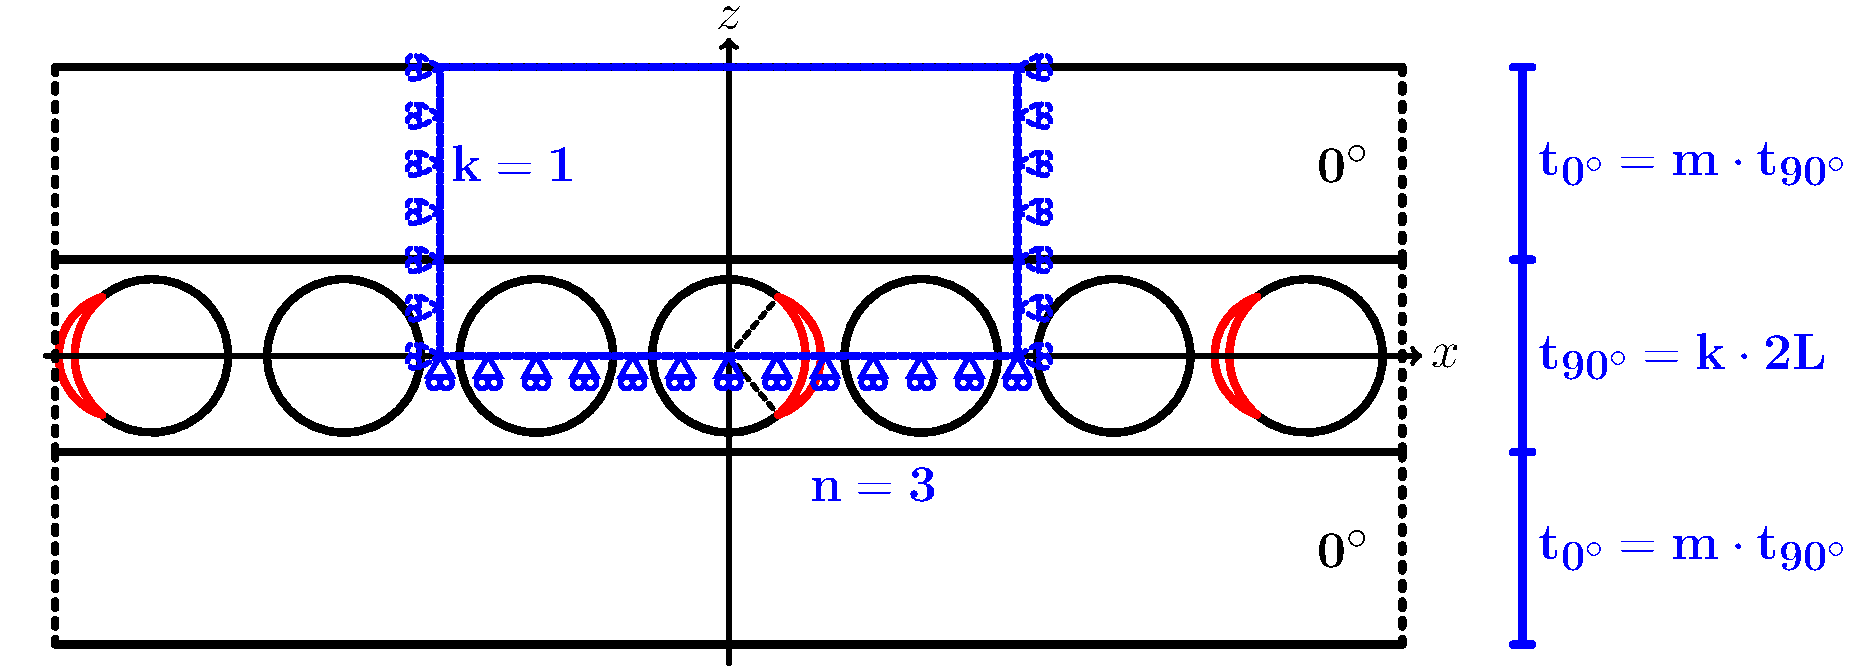
\includegraphics[height=0.225\textheight]{thinPly.pdf}
\caption{Models of $\left[0_{m\cdot 1\cdot2L}^{\circ},90_{1\cdot2L}^{\circ},0_{m\cdot 1\cdot2L}^{\circ}\right]$ laminates with an ultra-thin $90^{\circ}$ layer, where the $90^{\circ}$ ply is made up by a single ``row'' of fibers. Debonds are repeating at different distances, measured in terms of the number $n-1$ of fully bonded fibers appearing between two consecutive debonds. $2L$ is the thickness of one-fiber row.}\label{fig:laminateModelsA}
\end{figure}

All the RUCs present regular microstructures with fibers placed according to a square-packing configuration characterized by the repetition of the same one-fiber unit cell of size $2L\times2L$, where $L$ is a function of the fiber volume fraction $V_{f}$ and the fiber radius according to

\begin{equation}\label{eq:LVf}
L=\frac{R_{f}}{2}\sqrt{\frac{\pi}{V_{f}}}.
\end{equation}

The choice of a square-packing configuration with a controlled number of fibers is motivated by the fact that our objective is to determine the effect of different geometrical and mechanical factors on debond Energy Release Rate, such as fiber volume fraction, the presence of undamaged and partially debonded fibers, the presence of the $0^{\circ}/90^{\circ}$ interface. The use of a regular microstructure allows us to isolate and identify the different contributions, which would be otherwise ``smeared out'' with the use of randomized distribution with a large number of fibers. Each fiber in the model has the same radius $R_{f}$, equal to $1\ \mu m$. This specific value has no physical meaning per se and it has been selected for simplicity. It is useful to observe that, in a linear elastic solution subject to non-holonomic constraints as the one described in the present article, the ERR is proportional to the geometrical dimensions of the model and thus re-evaluation of the ERR for fibers of any size requires just a multiplication. Furthermore, it is worth to point out that $V_{f}$ is the same in the one-fiber unit and in the overall RUC, i.e. no clustering of fibers is considered.\\

\begin{figure}[!htb]
\centering
        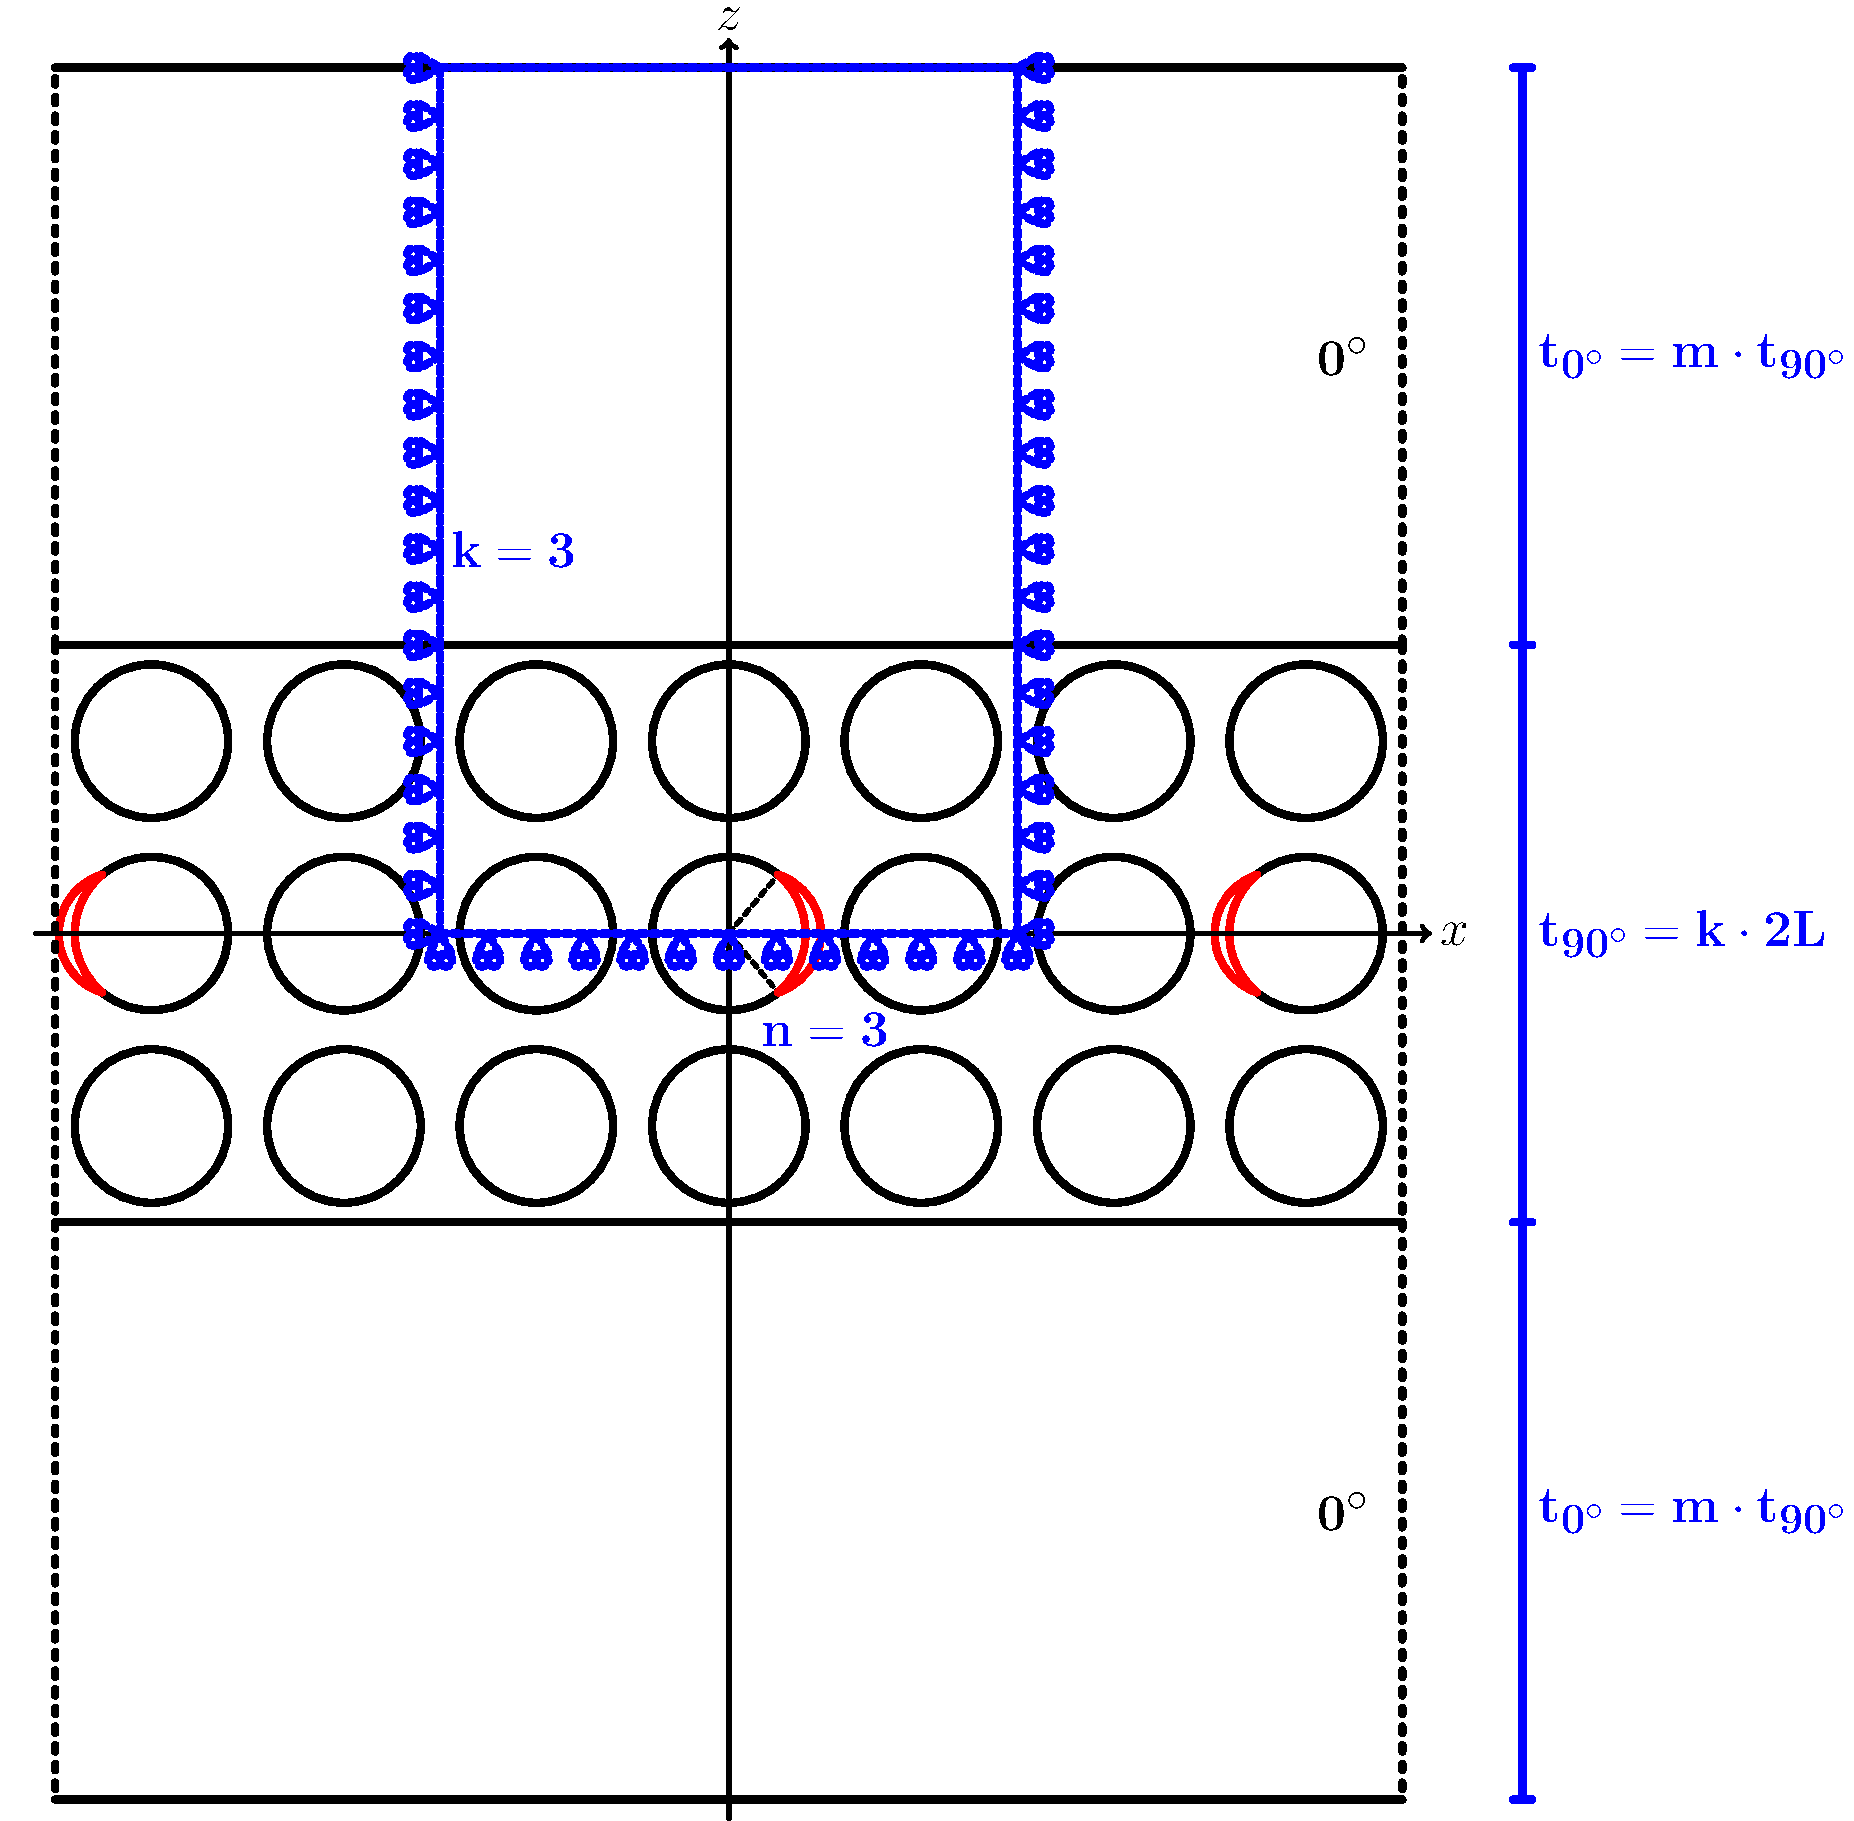
\includegraphics[height=0.425\textheight]{ThickPly.pdf}
   %    \caption{Mutiple rows of fibers with a debond appearing every $n$ fibers within the central row: model $n\times k-free$ ($n=3$ and $k=3$ in the figure).}\label{subfig:thickply}
\caption{Models of $\left[0_{m\cdot k\cdot2L}^{\circ},90_{k\cdot2L}^{\circ},0_{m\cdot k\cdot2L}^{\circ}\right]$ laminates with a $90^{\circ}$ layer of variable thickness, determined by the number $k$ of ``rows'' of fibers along the vertical direction.  Debonds are repeating at different distances along the horizontal direction, measured in terms of the number $n-1$ of fully bonded fibers appearing between two consecutive debonds. $2L$ is the thickness of one-fiber row.}\label{fig:laminateModelsB}
\end{figure}

The thickness of the $90^{\circ}$ ply depends on the number $k$ of fiber rows present across the thickness (the vertical or $z$ direction in Figures~\ref{fig:laminateModelsA} and~\ref{fig:laminateModelsB}) according to

\begin{equation}\label{eq:t90}
t_{90^{\circ}}=k\cdot2L.
\end{equation}

On the other hand, the thickness of $0^{\circ}$ layers can be assigned freely as a multiple of the $90^{\circ}$ ply thickness as

\begin{equation}\label{eq:t90}
t_{0^{\circ}}=m\cdot t_{90^{\circ}}
\end{equation}

where $m$ is an arbitrary integer. Thus, the thickness ratio $m$ represents one additional parameter for the investigation.\\
%In the RUCs proposed, we consider the $90^{\circ}$ ply with debonds as a series of stacked damaged and undamaged fiber rows, each row with only one fiber in the thickness direction.
In the following, let us consider in-plane coordinates $x$ and $y$, and assume that the laminate $0^{\circ}$-direction is aligned with the $x$-axis. In the presence of a load in the $x$-direction, the strain in the $y$-direction is small, due to the very small Poisson's ratio of the laminate. Debonds are present only in the $90^{\circ}$ layer and are considered to be significantly longer in the fiber direction than in the arc direction~\cite{Zhang1997}. Therefore we use 2D models under the assumption of plane strain, defined in the $x-z$ section of the composite. The study presented in this paper thus applies to long debonds and its focus is on understanding the mechanisms of growth along their arc direction. The laminates are assumed to be subject to tensile strain, which is applied in the form of a constant displacement in the $x$-direction along both vertical boundaries of the RUC as shown in  Figure~\ref{fig:modelschem}.\\
We assume damage to be present only in the central ``row'' of fibers of the $90^{\circ}$ layer in the form of multiple debonds appearing at different regular intervals along the loading (horizontal) direction. The number of fibers $n$ present in the horizontal direction of the RUC (Figures~\ref{fig:laminateModelsA} and~\ref{fig:laminateModelsB}) controls the distance, in terms of fully bonded fibers, between consecutive debonds: if the RUC has $n$ fibers in the horizontal direction, two consecutive debonds are separated by $n-1$ undamaged fibers. The RUCs considered are thus Representative Volume Elements (RVEs) of cross-ply laminates with a certain distribution of debonds in the middle $90^{\circ}$ layer.\\
In summary, the models are differentiated by: first, the spacing between debonds along the horizontal direction in the $90^{\circ}$ layer, which corresponds to the number $n$ of fibers in the RUC's horizontal direction; second, the thickness of the middle $90^{\circ}$ ply measured in terms of the number $k$ of fiber rows in the vertical direction; third, the factor $m$ which provides the thickness of $0^{\circ}$ layers as a multiple of the $90^{\circ}$ ply thickness. It thus seems natural to introduce a common notation for the RUCs as $n\times k-m\cdot t_{90^{\circ}}$.\\
An additional family of RUCs is considered, in which: only one partially debonded fiber is present; the $0^{\circ}$ layer is absent; different combinations of displacement boundary conditions are applied to the upper surface. The application of coupling of horizontal displacements $u_{x}$ along the right and left sides allows for repetition along the horizontal direction. When the upper boundary of the RUC is left free, we define the $1\times 1-free$ model. If coupling of the vertical displacements $u_{z}$ is applied to the upper boundary (coupling condition), we define instead the $1\times 1-coupling$ model. In the case a linear distribution of the horizontal displacement $u_{x}$ is applied to the upper boundary (H-condition), the model is refered to as $1\times 1-H$. Finally, when the linear distribution of the horizontal displacement $u_{x}$ is superimposed to the condition of coupling of the vertical displacements $u_{z}$ on the upper boundary, we have the $1\times 1-coupling+H$. Further details about this family of RUCs and the corresponding laminate RVE can be found in~\cite{DiStasio2019}.

%% 2.2 Models of Representative Volume Element (RVE)

\subsection{Description of modelled Representative Volume Elements (RVEs)}\label{subsec:rve}

The first family of Representative Volume Elements (RVEs) is represented in Figure~\ref{fig:laminateModelsA}. It represents a set of $\left[0_{m\cdot 1\cdot2L}^{\circ},90_{1\cdot2L}^{\circ},0_{m\cdot 1\cdot2L}^{\circ}\right]$ laminates with an ultra-thin $90^{\circ}$ layer, constituted by a single row of fibers across the thickness. Debonds appear at regular intervals measured in terms of number $n-1$ of fully bonded fibers present between them, which in turn correspond to the number of fibers along the horizontal direction of the RVE as highlighted in Fig.~\ref{fig:laminateModelsA}. They are thus the $n\times1-m\cdot t_{90^{\circ}}$ models, where $m=1,10$ and $n$ is an integer $\geq1$ ($n=1$ corresponds to the case of a debond appearing on all the fibers in the central $90^{\circ}$ layer). These models are geometrically extreme, but allow to focus on the interaction between debonds and the inter-ply $0^{\circ}/90^{\circ}$ interface. Furthermore, the \emph{spread tow} technology is today capable of producing cross-ply laminates with the central $90^{\circ}$ layer thickness only $4-5$ times the fiber diameter, as shown for example in~\cite{Saito2012}, which may in future give practical relevance even to such extreme case.\\
The second set of models considers instead cross-ply laminates with a central $90^{\circ}$ ply of variable thickness, measured in terms of number $k$ of fiber rows ``stacked'' in the vertical direction in Figure~\ref{fig:laminateModelsB}. Once again, debonds appear in the central row only at regular intervals measured in terms of number $n-1$ of fully bonded fibers present between them, as highlighted in Fig.~\ref{fig:laminateModelsB}. These models are thus the $n\times k-m\cdot t_{90^{\circ}}$ models, where $m=1,10$, $k>1$ and $n$ is an integer $\geq1$ ($n=1$ corresponds to the case of a debond appearing on all fibers of the central fiber row in the $90^{\circ}$ layer). By increasing the number $n$ of fibers in the horizontal direction in the RUC, decreasing levels of damage (debonds spaced further apart and the interaction between debonds becomes less important) are considered to be present in the laminate. By increasing the number $k$ of fiber rows, the thickness of the $90^{\circ}$ layer is increased and the effect of the relative proximity of the inter-ply $0^{\circ}/90^{\circ}$ interface can thus be studied. Finally, by increasing the factor $m$, the thickness of the $0^{\circ}$ layers is increased for a given thickness of the $90^{\circ}$, which allows the investigation of the $0^{\circ}$ ply-block effect~\cite{Teixeira2016}.

%% 2.3 Finite Element (FE) discretization

\subsection{Finite Element (FE) discretization}

The RUCs are discretized and solved with the Finite Element Method (FEM) using the commercial FEM package Abaqus~\cite{abq12}. The total length and height of a RUC are determined by the number of fibers $n$ in the horizontal direction, the number of fiber rows $k$ across the thickness and the thickness ratio $m$ (see Sec.~\ref{subsec:names} and Sec.~\ref{subsec:rve}). The debond appears symmetrically with respect to the $x$ axis (see Fig.~\ref{fig:modelschem}) and we characterize it with the angular size $\Delta\theta$ (the full debond size is thus $2\Delta\theta$). In the case of large debond sizes ($\geq 60^{\circ}-80^{\circ}$), a region of size $\Delta\Phi$ to be determined by the solution itself appears at the crack tip. In this region, called the \emph{contact zone}, the crack faces are in contact and slide on each other. Due to existence of the contact zone, frictionless contact is considered between the two crack faces to avoid interpenetration and allow free sliding. Symmetry with respect to the $x$ axis is applied on the lower boundary. Kinematic coupling on the $x$-displacement is applied along the left and right boundaries of the model in the form of a constant $x$-displacement $\pm\bar{\varepsilon}_{x} nL$, corresponding to laminate $x$-strain $\bar{\varepsilon}_{x}$ equal to $1\%$. The bimaterial interface crack problem belongs to the class of \emph{receding contact}~\cite{Paris1996,Garrido1991}, i.e. such that the contact zone in the final configuration is smaller than in the initial one. It was shown that this class of problems has some peculiar properties~\cite{Keer1972,Tsai1974}, which are valid both with and without friction at the interface~\cite{Paris1996,Garrido1991}: size and shape of the contact zone remain the same upon a change in the magnitude of the applied load; only a change in the disposition of the applied load causes a change in the size and shape of the contact zone; displacements, stresses and strains (and consequently, Energy Release Rate) are directly proportional to the value of the applied load. Thus, although our interest is to compare the relative magnitude of Mode I and Mode II ERR among different configurations, the results presented could be used to compute the ERR at different levels of the applied strain through a simple multiplication.\\

\begin{figure}[!htb]
\centering
        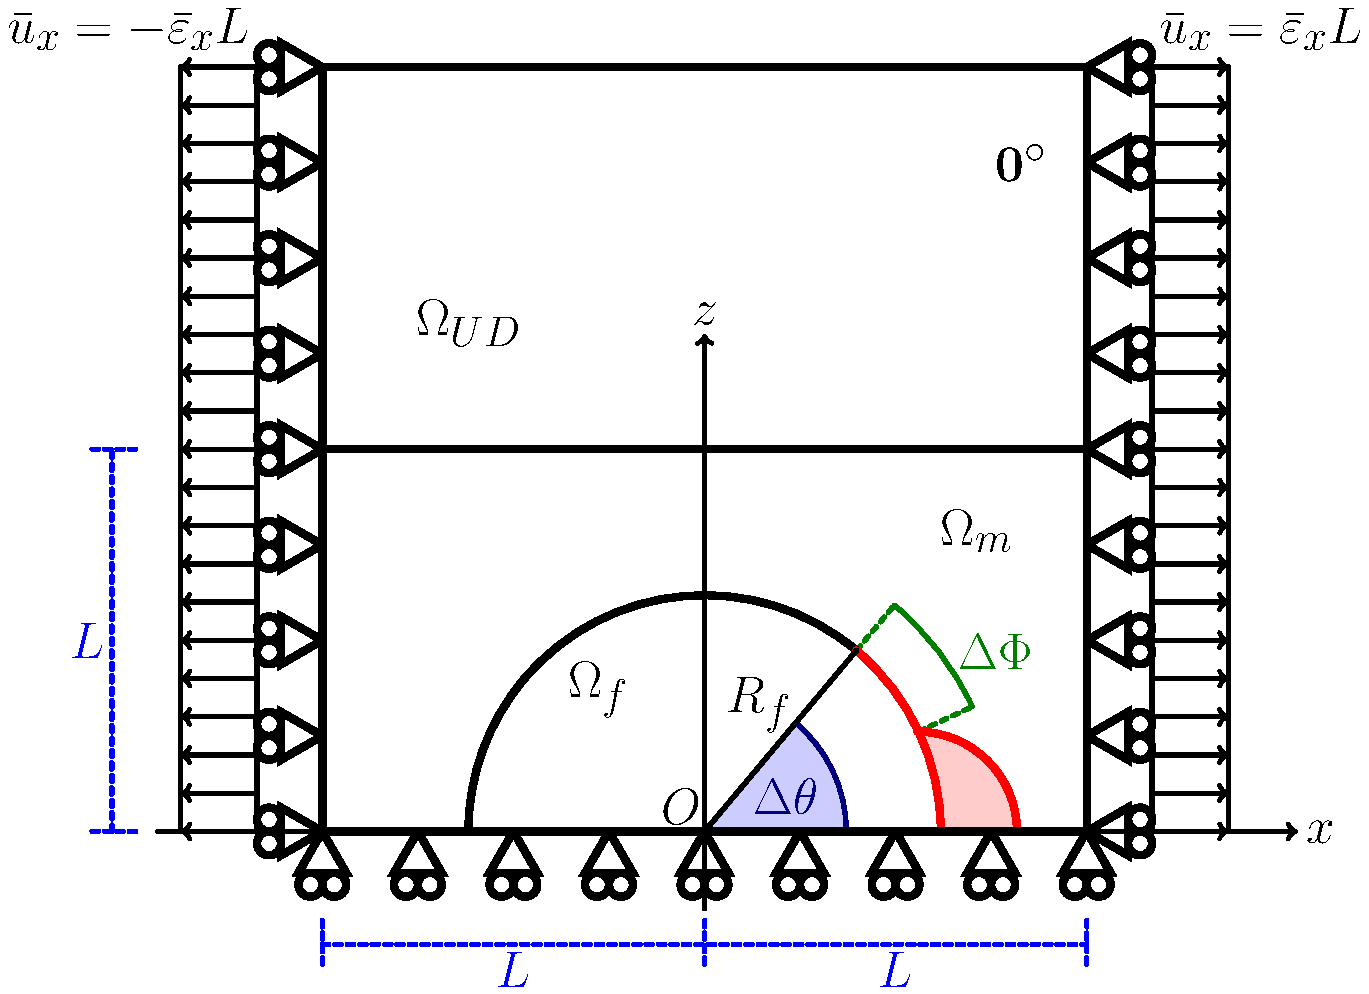
\includegraphics[height=0.375\textheight]{RUC.pdf}
\caption{Schematic of the model with its main parameters.}\label{fig:modelschem}
\end{figure}

The FEM model is discretized using second order, 2D, plane strain triangular (CPE6) and rectangular (CPE8) elements. In the crack tip neighborhood, a refined regular mesh of quadrilateral elements with almost unitary aspect ratio is needed to ensure a correct evaluation of the ERR. The angular size $\delta$ of an element in this refined region close to the crack tip is by design equal to $0.05^{\circ}$. The crack faces are modeled as element-based surfaces with a frictionless small-sliding contact pair interaction. The Mode I, Mode II and total Energy Release Rates (ERRs) (respectively $G_{I}$, $G_{II}$ and $G_{TOT}$) represent the main result of the numerical analysis. They are computed using the VCCT~\cite{Krueger2004} implemented in a custom Python routine. Glass fiber and epoxy are considered throughout this article, and it is assumed that their response always lies in the linear elastic domain. The effective UD properties are computed using Hashin's Concentric Cylinder Assembly model~\cite{Hashin1983} with the self-consistency scheme for the out-of-plane shear modulus of Christensen~\cite{Christensen1979}. The properties used are listed in Table~\ref{tab:phaseprop}. The model was validated with respect to BEM results of~\cite{Paris2007,Sandino2016}; considerations about the order of accuracy can be found in~\cite{DiStasio2019}.

\begin{table}[!h]
 \centering
 \caption{Summary of mechanical properties of fiber, matrix and UD layer (GF: glass fiber; EP: epoxy; UD: glass-fiber/epoxy uni-directional properties).}%$E$ stands for Young's modulus, $\mu$ for shear modulus and $\nu$ for Poisson's ratio. Indexes $L$ and $T$ stand respectively for \emph{longitudinal} and \emph{transverse}.}
 \begin{tabular}{ccccccc}
\small& \small\textbf{$V_{f}\left[\%\right]$}\  &\small \textbf{$E_{L}\left[GPa\right]$}\ & \small\textbf{$E_{T}\left[GPa\right]$}\  & \small\textbf{$G_{LT}\left[GPa\right]$} &\small\textbf{$\nu_{LT}\left[-\right]$} &\small \textbf{$\nu_{TT}\left[-\right]$} \\
\midrule
\small GF &\small-   &\small 70.0 &\small 70.0  &\small 29.2 &\small 0.2  &\small 0.2\\
\small EP    &-&\small 3.5 &\small 3.5   &\small 1.25 &\small  0.4&\small 0.4\\
\small UD&\small60.0&\small43.442&\small13.714&\small 4.315&\small 0.273&\small0.465\\
\end{tabular}
\label{tab:phaseprop}
\end{table}

%%%%%%%%%%%%%%%%%%%%%%%%%%%%%%%%%%%%%%%%%%%%%%%%%%%%%%%%%%%%%%%%%%%
% 3. RESULTS AND DISCUSSION
%%%%%%%%%%%%%%%%%%%%%%%%%%%%%%%%%%%%%%%%%%%%%%%%%%%%%%%%%%%%%%%%%%%

\section{Results \& Discussion}

\subsection{Effect of the proximity of the $0^{\circ}/90^{\circ}$ interface and of the thickness of the $0^{\circ}$ layer on debond ERR for highly interactive debonds}\label{subsec:thickness}

We first focus our attention on the model $1\times 1-m\cdot t_{90^{\circ}}$, which represents a particular case of the family $n\times 1-m\cdot t_{90^{\circ}}$. It corresponds to a cross-ply laminate in which the central $90^{\circ}$ ply is constituted by only one fiber row, in which each fiber possesses a debond appearing on alternating sides. The model thus represents an extreme idealization, in the sense that: first, the central $90^{\circ}$ layer is the thinniest that can be conceived, which allows us to investigate the direct effect of the proximity of the $0^{\circ}/90^{\circ}$ interface on debond ERR; second, a very particular damage state is present for which every fiber is partially debonded from the sorrounding matrix, corresponding to the most severe damage state that can occur in the $90^{\circ}$ ply when considering debonds as the only mechanism of damage. We are thus focusing on the presence of the $0^{\circ}/90^{\circ}$ interface and on the thickness of the $0^{\circ}$ layer, by considering the ratio $m=\frac{t_{0^{\circ}}}{t_{90^{\circ}}}$ of ply thicknessess as a free parameter.\\

\begin{figure}[!htb]
\centering
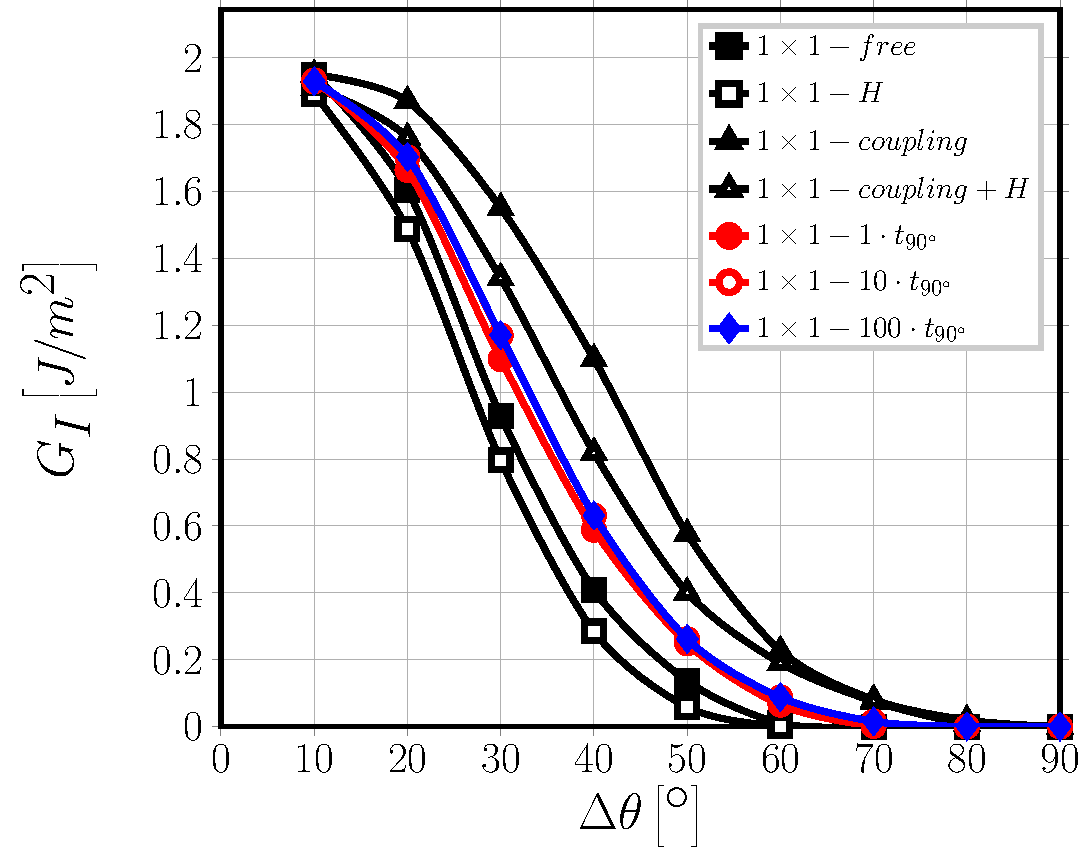
\includegraphics[height=0.375\textheight]{1x1-i-vf60-GI.pdf}
\caption{Effect of the proximity of the $0^{\circ}/90^{\circ}$ interface and of the thickness of the $0^{\circ}$ layer on Mode I ERR: models $1\times 1-free$, $1\times 1-H$, $1\times 1-coupling$, $1\times 1-coupling+H$ and $1\times 1-m\cdot t_{90^{\circ}}$. $V_{f}=60\%$, $\bar{\varepsilon}_{x}=1\%$.}\label{fig:thicknessGI}
\end{figure}

In Figures~\ref{fig:thicknessGI} and~\ref{fig:thicknessGII} it is possible to observe respectively the Mode I and Mode II ERR for models $1\times 1-m\cdot t_{90^{\circ}}$ with $m=1,10,100$. Mode I ERR is practically unaffected by the $0^{\circ}$ layer thickness, only a marginal increase $\leq1\%$ can be seen when $m$ is increased from $1$ to $10$. No further observable change is present when $m$ is increased to $100$. Moreover, the contact zone onset, which corresponds to the first value of $\Delta\theta$ such that $G_{I}=0$, is always equal to $70^{\circ}$ irrespective of the value of $m$. A more remarkable, albeit small, effect of the $0^{\circ}$ layer thickness can be observed for Mode II when $m$ is increased from $1$ to values $\geq10$. For open cracks, i.e. when no contact zone is present and thus $\Delta\theta$ is smaller than $70^{\circ}$, increasing the $0^{\circ}$ layer thickness causes a reduction of Mode II ERR; while for closed cracks, when a contact zone is present and $\Delta\theta>70^{\circ}$, the increase in thickness leads to an increase in ERR.\\

\begin{figure}[!htb]
\centering
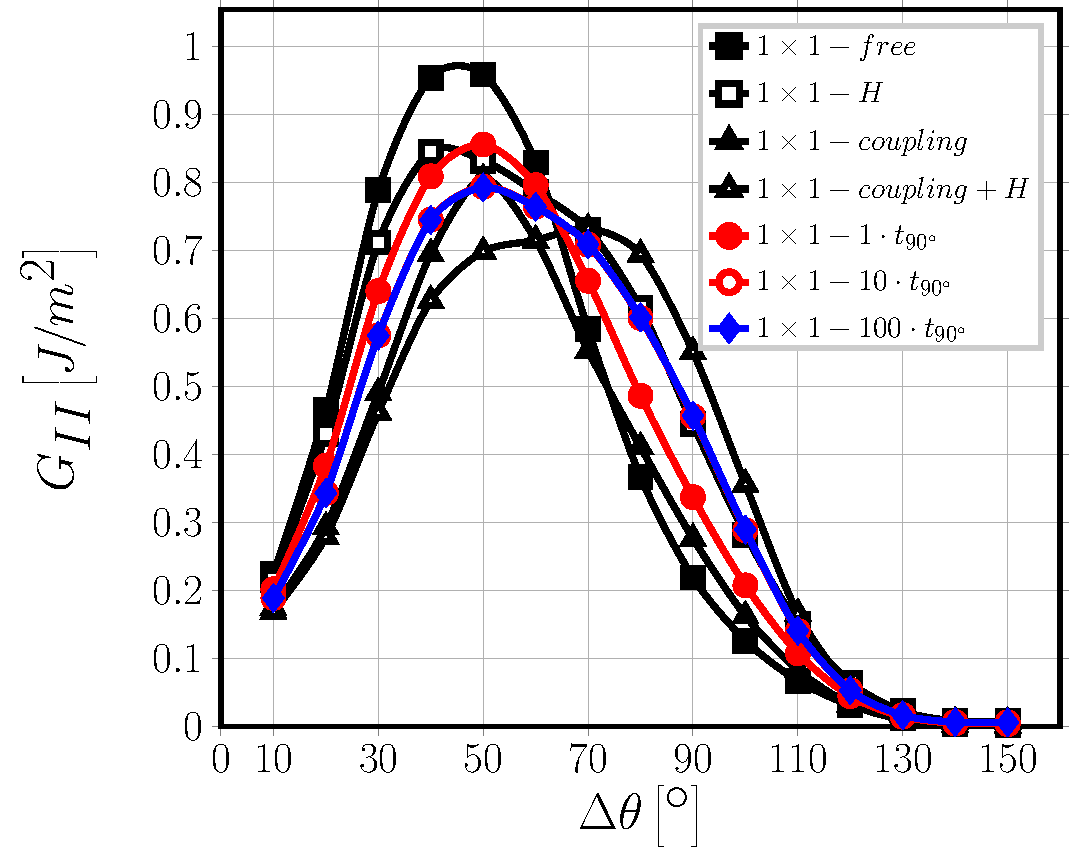
\includegraphics[height=0.375\textheight]{1x1-i-vf60-GII.pdf}
\caption{Effect of the proximity of the $0^{\circ}/90^{\circ}$ interface and of the thickness of the $0^{\circ}$ layer on Mode II ERR: models $1\times 1-free$, $1\times 1-H$, $1\times 1-coupling$, $1\times 1-coupling+H$ and $1\times 1-m\cdot t_{90^{\circ}}$. $V_{f}=60\%$, $\bar{\varepsilon}_{x}=1\%$.}\label{fig:thicknessGII}
\end{figure}

In order to understand the interaction mechanism between the $0^{\circ}/90^{\circ}$ interface and the debond, Mode I and Mode II ERR are reported respectively in Figures~\ref{fig:thicknessGI} and~\ref{fig:thicknessGII} for models $1\times 1-free$, $1\times 1-H$, $1\times 1-coupling$ and $1\times 1-coupling+H$. These RUCs all present equivalent boundary conditions and it is here useful to recall their characteristics: in model $1\times 1-free$ the upper bounday is left free; coupling conditions on the vertical displacements $u_{z}$ are applied to the upper boundary in model $1\times 1-coupling$ (coupling condition); in model $1\times 1-H$ a linearly distributed horizontal displacement $u_{x}$ is applied to the upper boundary (H-condition); in model $1\times 1-coupling+H$ coupling conditions on the vertical displacements $u_{z}$ and a linearly distributed horizontal displacement $u_{x}$ are imposed together on the upper boundary. Given that the presence of a $0^{\circ}$ layer provides two constraints: first, it tends to keep the $90^{\circ}$ layer boundary straight; second, it forces a more homogeneous horizontal displacement at the $90^{\circ}$ layer boundary; the equivalent boundary conditions of $1\times 1-coupling$, $1\times 1-H$ and $1\times 1-coupling+H$ represent an extreme case respectively of the first constraint ($1\times 1-coupling$), the second constraint ($1\times 1-H$) and the two together ($1\times 1-coupling+H$). The case $1\times 1-free$ constitutes instead the base case (absence of $0^{\circ}$ layer), on which comparisons are built.\\
Observing Figure~\ref{fig:thicknessGI}, it is possible to notice that the values of $G_{I}$ for the $1\times 1-free$ and the $1\times 1-coupling$ models represent respectively a lower and an upper bound for the $1\times 1-m\cdot t_{90^{\circ}}$ RVEs: this is true with respect to the value of $G_{I}$ as well as of contact zone onset ($60^{\circ}$ for  $1\times 1-free$, $70^{\circ}$ for $1\times 1-m\cdot t_{90^{\circ}}$, $80^{\circ}$ for $1\times 1-coupling$). When the H-condition is added to the $1\times 1-free$ and the $1\times 1-coupling$ models, thus obtaining the $1\times 1-H$ and $1\times 1-coupling+H$ models, $G_{I}$ decreases while the value of $\Delta\theta$ at contact zone onset remains unchanged ($60^{\circ}$ for  $1\times 1-free$ and $1\times 1-H$, $80^{\circ}$ for $1\times 1-coupling$ and $1\times 1-coupling+H$). Moreover, it is possible to observe that the values of $G_{I}$ of $1\times 1-coupling+H$ are much closer to but always greater than those of $1\times 1-m\cdot t_{90^{\circ}}$ RVEs, thus constituting a more representative upper bound for the latter.\\
Analogous considerations are drawn with regard to Mode II (see Fig.~\ref{fig:thicknessGII}). For small debonds, $\Delta\theta\leq30^{\circ}$, no significant difference in $G_{II}$ can be seen between $1\times 1-free$ and $1\times 1-H$ and between $1\times 1-coupling$ and $1\times 1-coupling+H$ in this region. With respect to $1\times 1-m\cdot t_{90^{\circ}}$ RVEs, the first pair ($1\times 1-free$ and $1\times 1-H$) represents the lower bound while the second pair ($1\times 1-coupling$ and $1\times 1-coupling+H$) the upper bound. For $30^{\circ}<\Delta\theta\leq60^{\circ}$, $1\times 1-H$ and $1\times 1-coupling+H$ provide significantly lower values of $G_{II}$ than respectively $1\times 1-free$ and $1\times 1-coupling$. $G_{II}$ values of $1\times 1-H$ are very close to $1\times 1-1\cdot t_{90^{\circ}}$, even coincident for $\Delta\theta=60^{\circ}$. On the other hand, $G_{II}$ values of $1\times 1-coupling$ are very close to $1\times 1-m\cdot t_{90^{\circ}}$ with $m\geq10$ and even coincident for $\Delta\theta=50^{\circ}$. For $60^{\circ}<\Delta\theta\leq110^{\circ}$, the situation changes. $1\times 1-free$ and $1\times 1-coupling$ provides values of $G_{II}$ close to each other, even coincident for $\Delta\theta=70^{\circ}$. Values of $G_{II}$ of $1\times 1-H$ and $1\times 1-coupling+H$ are significantly larger than both $1\times 1-free$ and $1\times 1-coupling$. Furthermore, $G_{II}$ values of $1\times 1-H$ coincide with those of $1\times 1-m\cdot t_{90^{\circ}}$ with $m\geq10$. Mode II ERR of $1\times 1-1\cdot t_{90^{\circ}}$ is instead close, but not coincident, to that of $1\times 1-coupling$. For $\Delta\theta>110^{\circ}$, $G_{II}$ is the same for all models and reaches $0$ at a debond size of around $130^{\circ}$.\\
These results help to understand the effect of the $0^{\circ}/90^{\circ}$ interface on debond ERR. Two constraining mechanisms are present in the case of $0^{\circ}/90^{\circ}$ interface that are absent in the free surface case: first, the boundary of the $90^{\circ}$ layer remains straighter (effect modelled by the coupling condition in $1\times 1-coupling$); second, the $x$-strain on the $90^{\circ}$ layer boundary is more uniform (effect modelled by the H-condition in $1\times 1-H$).\\
%The presence of the stiff homogenized $0^{\circ}$ layer causes the matrix placed relatively far from the fiber (close to the interface) to contract less than it would do in the presence of a free surface due to its relatively high Poisson's ratio. In the free surface case, the contraction ($z$-strain) would be different at different positions along the $x$-axis as the $x$-strain is not uniform; in the presence of the $0^{\circ}/90^{\circ}$ interface, the $x$-strain is instead more homogenuous and, consequently, the $z$-strain as well.\\
For small debonds ($\Delta\theta<60^{\circ}-70^{\circ}$), the presence of the $0^{\circ}/90^{\circ}$ interface causes an increase of $G_{I}$ and a decrease of $G_{II}$ with respect to the free surface case. For Mode I, the fact that the $90^{\circ}$ layer boundary remains straight (coupling condition) forces the debond to open more than in the free case, thus increasing $G_{I}$. However, the uniformity of the $x$-strain on the $90^{\circ}$ layer boundary reduces the local (in the debond neighborhood) $x$-strain magnification and contains the increase in $G_{I}$. This corresponds in Figure~\ref{fig:thicknessGI} to the fact that Mode I ERR for $1\times1-m\cdot t_{90^{\circ}}$ is always higher than $1\times1-free$ but lower than $1\times1-coupling$, and it is best approximated by $1\times1-coupling+H$. For Mode II in the case of small debonds, the presence of the $0^{\circ}$ layer  keeps the $0^{\circ}/90^{\circ}$ interface straighter and reduces the vertical contraction of the matrix, which contributes for the most part to Mode II in this range, thus leading to a decrease of $G_{II}$. The small effect of $0^{\circ}$ layer thickness on Mode II (Fig.~\ref{fig:thicknessGII}) can be explained in terms of local bending stiffness: a thinner $0^{\circ}$ layer ($\frac{t_{0^{\circ}}}{t_{90^{\circ}}}=1$) does not keep the $90^{\circ}$ layer boundary as straight as thicker $0^{\circ}$ layers ($\frac{t_{0^{\circ}}}{t_{90^{\circ}}}\geq10$). In the case $\frac{t_{0^{\circ}}}{t_{90^{\circ}}}=1$, the $90^{\circ}$ layer boundary deforms in a way that is similar to the free surface case, but smaller in magnitude. This corresponds to the fact that for $\Delta\theta<60^{\circ}-70^{\circ}$, in Figure~\ref{fig:thicknessGII}: $1\times1-1\cdot t_{90^{\circ}}$ is best approximated by $1\times1-H$ (curved $90^{\circ}$ layer boundary but uniform $x$-strain at the $90^{\circ}$ layer boundary that disfavors $G_{II}$), $1\times1-m\cdot t_{90^{\circ}},m\geq10$ is best approximated by $1\times1-coupling$ (straight $90^{\circ}$ layer boundary).\\
For debonds larger than $70^{\circ}$, the presence of the $0^{\circ}/90^{\circ}$ interface causes an increase of $G_{II}$ with respect to the free surface case. The uniform $x$-strain distribution on the $90^{\circ}$ layer boundary determined by the presence of the $0^{\circ}$ layer causes, with respect to the free case, the matrix $x$-strain to be higher in the $x\sim0$ neighborhood and lower around $x\sim\pm L$, in order to keep the average $\varepsilon_{x}$ at $1\%$. Given that for large debonds Mode II ERR is determined mostly by the magnitude of the $x$-strain gap (between the matrix $x$-strain and the fiber $x$-strain), an increase of $G_{II}$ is thus observed in the presence of the $0^{\circ}/90^{\circ}$ interface. Again, the observed effect of the $0^{\circ}$ layer thickness on Mode II for $\Delta\theta>60^{\circ}-70^{\circ}$ (Fig.~\ref{fig:thicknessGII}) can be discussed in terms of local $0^{\circ}$ layer bending stiffness. In the free case, it is the curvature of the material around the fiber that causes the $x$-strain reduction and thus a lower $G_{II}$. Thicker $0^{\circ}$ layers ($\frac{t_{0^{\circ}}}{t_{90^{\circ}}}\geq10$) prevent this $90^{\circ}$ boundary deformation to a greater extent than the thinner $t_{0^{\circ}}=t_{90^{\circ}}$ case: the $x$-strain (and thus $G_{II}$) increase is greater for $\frac{t_{0^{\circ}}}{t_{90^{\circ}}}\geq10$ than $\frac{t_{0^{\circ}}}{t_{90^{\circ}}}=1$.

\subsection{Effect of the proximity of the $0^{\circ}/90^{\circ}$ interface and of the thickness of the $0^{\circ}$ layer on non-interactive debonds in a one-fiber row $90^{\circ}$ ply}\label{subsec:debonddebondinter}

We turn now our attention to models $n\times 1-m\cdot t_{90^{\circ}}$, which correspond to a cross-ply laminate in which the central $90^{\circ}$ ply is constituted by only one fiber row where multiple partially debonded fibers are present with $n-1$ fully bonded fibers between them and debonds appear on alternating sides of consecutive damaged fibers (see Figure~\ref{fig:laminateModelsA}). %This class of models allows to study the effect of the presence of the $0^{\circ}$ layer and of its thickness on non-interactive debonds. 
As observed in a previous work~\cite{DiStasio2019}, the presence of fully bonded fibers between partially debonded ones in the loading direction has a strong effect on debond ERR and controls the interaction between debonds. When $n$ is increased, both Mode I and Mode II increase: the addition of stiffer elements, in the form of fully bonded fibers, increase the strain applied to the damaged unit and thus causes higher values of ERR. Looked from this perspective, i.e. moving from the most to the least severe state of damage, this effect is referred to as ``strain magnification''~\cite{DiStasio2019}. There seems to exist a characteristic distance, measured in terms of fully bonded fibers, above which a change in the number of undamaged fibers affects only marginally, or even not at all, debond ERR. This distance, generally $n\sim20$, marks the transition between a non-interactive solution ($n>20$) and an interactive one ($n<20$). The ``strain magnification'' effect thus represents the transition from the interactive to the non-interactive solution. If in Sec.~\ref{subsec:thickness} we studied the effect of the proximity of the $0^{\circ}/90^{\circ}$ interface and of the thickness of the $0^{\circ}$ layer on interactive debonds ($1\times 1-\dots$), we analyze in the present section the effect of the $0^{\circ}/90^{\circ}$ interface and of the $0^{\circ}$ layer thickness on non-interactive ones ($n\times 1-\dots\text{ with }n>20$).\\

\begin{figure}[!htb]
\centering
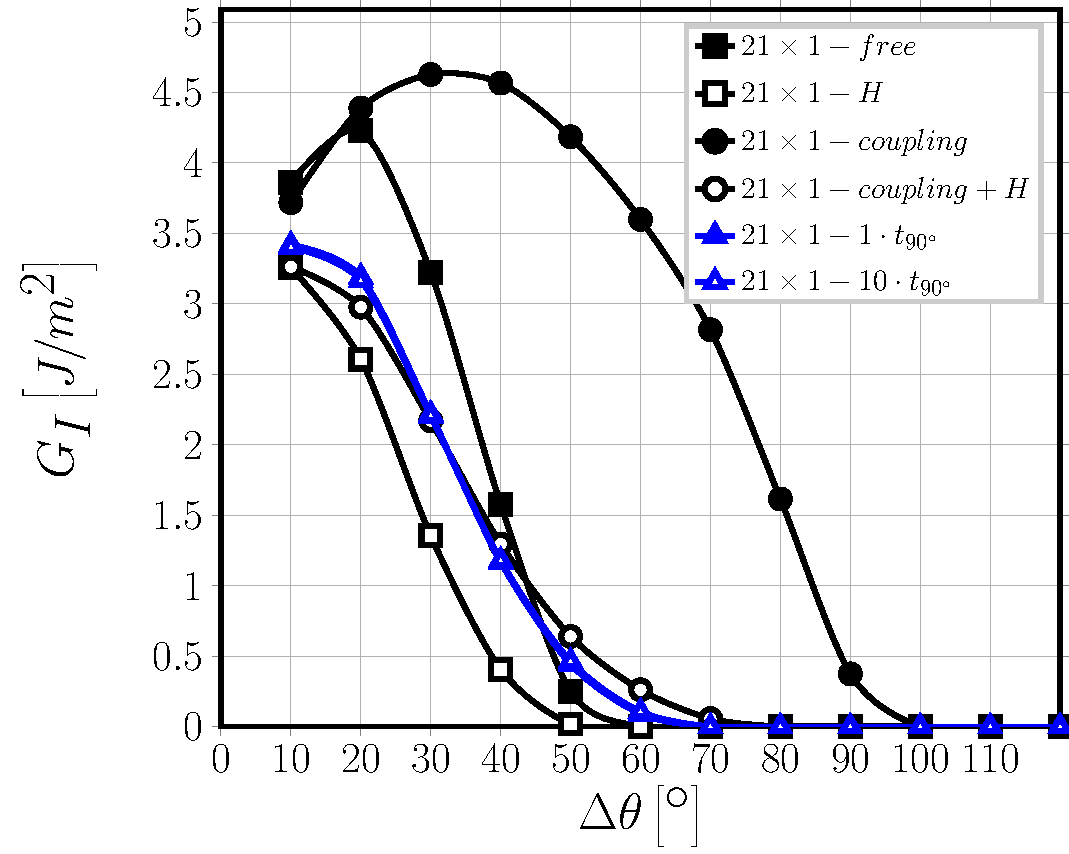
\includegraphics[height=0.375\textheight]{nx1-1-vf60-GI.pdf}
\caption{Effect of the presence of the $0^{\circ}$ layer on Mode I ERR of non-interactive debonds: models $21\times 1-free$, $21\times 1-H$, $21\times 1-coupling$, $21\times 1-coupling+H$, $21\times 1-1\cdot t_{90^{\circ}}$ and $21\times 1-10\cdot t_{90^{\circ}}$. $V_{f}=60\%$, $\bar{\varepsilon}_{x}=1\%$.}\label{fig:debonddebondGI}
\end{figure}

Comparing Fig.~\ref{fig:debonddebondGI} with Fig.~\ref{fig:thicknessGI} and Fig.~\ref{fig:debonddebondGII} with Fig.~\ref{fig:thicknessGII}, it is possible to observe how, as previously described, increasing the number of fully bonded fibers between consecutive debonds in the loading direction leads to an increase in Mode I and Mode II ERR. The peak $G_{I}$ increases from $1.93 \left[\frac{J}{m^{2}}\right]$ in $1\times 1-1\cdot t_{90^{\circ}}$ to $3.42 \left[\frac{J}{m^{2}}\right]$ in $21\times 1-1\cdot t_{90^{\circ}}$, while the peak $G_{II}$ from $0.86 \left[\frac{J}{m^{2}}\right]$ to $3.04 \left[\frac{J}{m^{2}}\right]$. The value of $\Delta\theta$ at contact zone onset remains however the same ($70^{\circ}$).\\
The effect of the $0^{\circ}$ layer thickness is instead non-existent: values of both $G_{I}$ and $G_{II}$ are coincident for $21\times 1-1\cdot t_{90^{\circ}}$ and $21\times 1-10\cdot t_{90^{\circ}}$.\\

\begin{figure}[!htb]
\centering
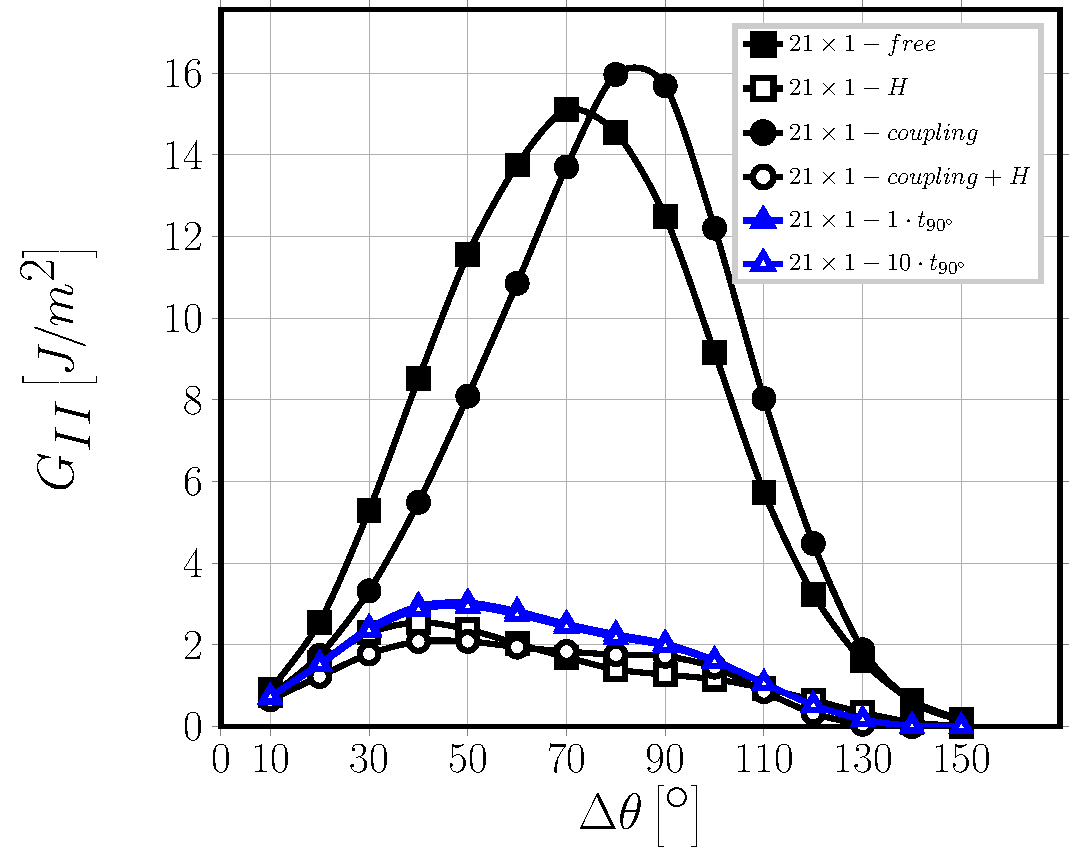
\includegraphics[height=0.375\textheight]{nx1-1-vf60-GII.pdf}
\caption{Effect of the presence of the $0^{\circ}$ layer on Mode II ERR of non-interactive debonds: models $21\times 1-free$, $21\times 1-H$, $21\times 1-coupling$, $21\times 1-coupling+H$, $21\times 1-1\cdot t_{90^{\circ}}$ and $21\times 1-10\cdot t_{90^{\circ}}$. $V_{f}=60\%$, $\bar{\varepsilon}_{x}=1\%$.}\label{fig:debonddebondGII}
\end{figure}

In agreement with the introductory considerations of this section and the results in~\cite{DiStasio2019}, it is possible to observe in Figures~\ref{fig:debonddebondGI} and~\ref{fig:debonddebondGII} that $21\times 1-free$ and $21\times 1-coupling$ (in which the horizontal displacement $u_{x}$ is left uncostrained on the upper boundary) show both the highest values of Mode I and Mode II ERR as well as the maximum increase with respect to the interactive case ($1\times 1-free$ and $1\times 1-coupling$). When the H-condition is applied to the upper boundary, thus constraining the magnitude of the strain magnification effect, both the magnitude of Mode I and Mode II ERR as well as their relative increase with respect to the interactive case are significantly reduced. $21\times 1-coupling+H$ represents, when considering both Mode I and Mode II ERR, the best approximation to the results of $21\times 1-m\cdot t_{90^{\circ}}$. The mechanisms at play are the same as in Sec.~\ref{subsec:thickness}: by keeping the $0^{\circ}/90^{\circ}$ interface straight (coupling condition), the $0^{\circ}$ layer favors an increase in $G_{I}$ and decrease in $G_{II}$ for small debonds and an increase in $G_{II}$ for large debonds; by applying a uniform $x$-strain on the $90^{\circ}$ layer boundary (H-condition), the $0^{\circ}$ layer promotes a more uniform $x$-strain in the $90^{\circ}$ layer and acts against the strain magnification effect, reducing debond ERR. Results in Fig.~\ref{fig:debonddebondGI} and Fig.~\ref{fig:debonddebondGII} show that the latter effect (H-condition) is dominant. It seems reasonable to conclude that debond growth is favored (i.e. debond ERR is higher) in the presence of strain or stress concentrations (as for example in the presence of a free surface or only coupling conditions on the vertical displacement), while more uniform strain and stress fields as those created by the proximity of the $0^{\circ}/90^{\circ}$ interface reduce both Mode I and Mode II ERR and thus tend to prevent debond growth.

\subsection{Effect of the presence of fiber rows with no damage on the debond-$0^{\circ}/90^{\circ}$ interface interaction}

After having investigated the effect of the proximity of the $0^{\circ}/90^{\circ}$ interface and of the thickness of the $0^{\circ}$ layer on debond ERR for different cases of debond-debond interaction in the same fiber row, we address in this section the effect of the presence of fiber rows with only fully bonded fibers between debonds and the $0^{\circ}/90^{\circ}$ interface. In other words, we are separating the debond from the $0^{\circ}/90^{\circ}$ interface by inserting rows of fully bonded fibers in between. We consider only the case $m=1$, i.e. $t_{0^{\circ}}=t_{90^{\circ}}$, given that increasing the $0^{\circ}$ layer thickness does not result in any remarkable effect on ERR as shown in Sec.~\ref{subsec:thickness} and Sec.~\ref{subsec:debonddebondinter}. Following the same philosophy of Sec.~\ref{subsec:thickness} and Sec.~\ref{subsec:debonddebondinter}, we analyze the effect of the presence of fiber rows with no damage on debond ERR: first, when the central fiber row possesses only partially debonded fibers, which represents the most severe damage state for these RUCs and the solution for interactive debonds (models $1\times k-1\cdot t_{90^{\circ}}$ in Figures~\ref{fig:1kGI} and~\ref{fig:1kGII}); second, the case of debonds separated by $n-1$ fully bonded fibers in the central fiber row, which corresponds to the least severe state of damage and to the solution for non-interactive debonds (models $21\times k-1\cdot t_{90^{\circ}}$ in Figures~\ref{fig:nkGI} and~\ref{fig:nkGII}).\\%Figures~\ref{fig:1kGI} and~\ref{fig:1kGII} thus show the effect on ERR of the presence of the $0^{\circ}$ ply in the case of non-interacting debonds (no strain magnification or crack shielding). If the distance between the $0^{\circ}/90^{\circ}$ interface and the debond is at least one fully bonded fiber, the presence of the $0^{\circ}$ ply does not influence debond ERR and no measurable difference can be observed between models $1\times k-free$ and $1\times k-1\cdot t_{90^{\circ}}$ for $k\geq1$.

\begin{figure}[!htb]
\centering
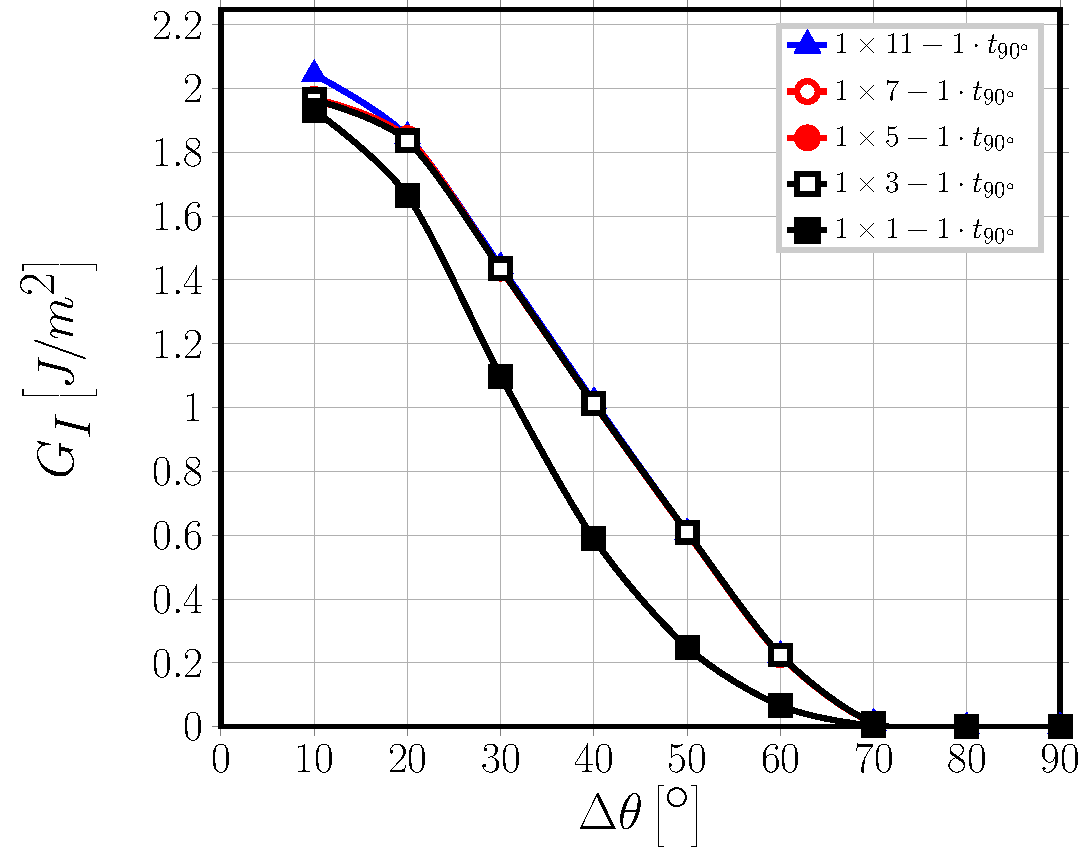
\includegraphics[height=0.375\textheight]{1xk-1-vf60-GI.pdf}
\caption{Effect of the presence of undamaged fiber rows in the $90^{\circ}$ layer on debond-$0^{\circ}/90^{\circ}$ interface interaction for Mode I ERR: models $1\times k-1\cdot t_{90^{\circ}}$. $V_{f}=60\%$, $\bar{\varepsilon}_{x}=1\%$.}\label{fig:1kGI}
\end{figure}

Observation of Fig.~\ref{fig:1kGI}, Fig.~\ref{fig:1kGII}, Fig.~\ref{fig:nkGI} and Fig.~\ref{fig:nkGII} reveals that no difference can be seen in Mode I and Mode II ERR by increasing the number $k$ of rows with undamaged fibers when $k\geq3$, which means that debond ERR does not change once at least $1$ row of undamaged fibers is present between the debond and the $0^{\circ}/90^{\circ}$ interface. A significant change is visible only when $k=1$, which means that no row of undamaged fibers is present between the debond and the $0^{\circ}/90^{\circ}$ interface. This change, from $k\geq3$ to $k=1$, corresponds in particular to a reduction of both $G_{I}$ and $G_{II}$.

\begin{figure}[!htb]
\centering
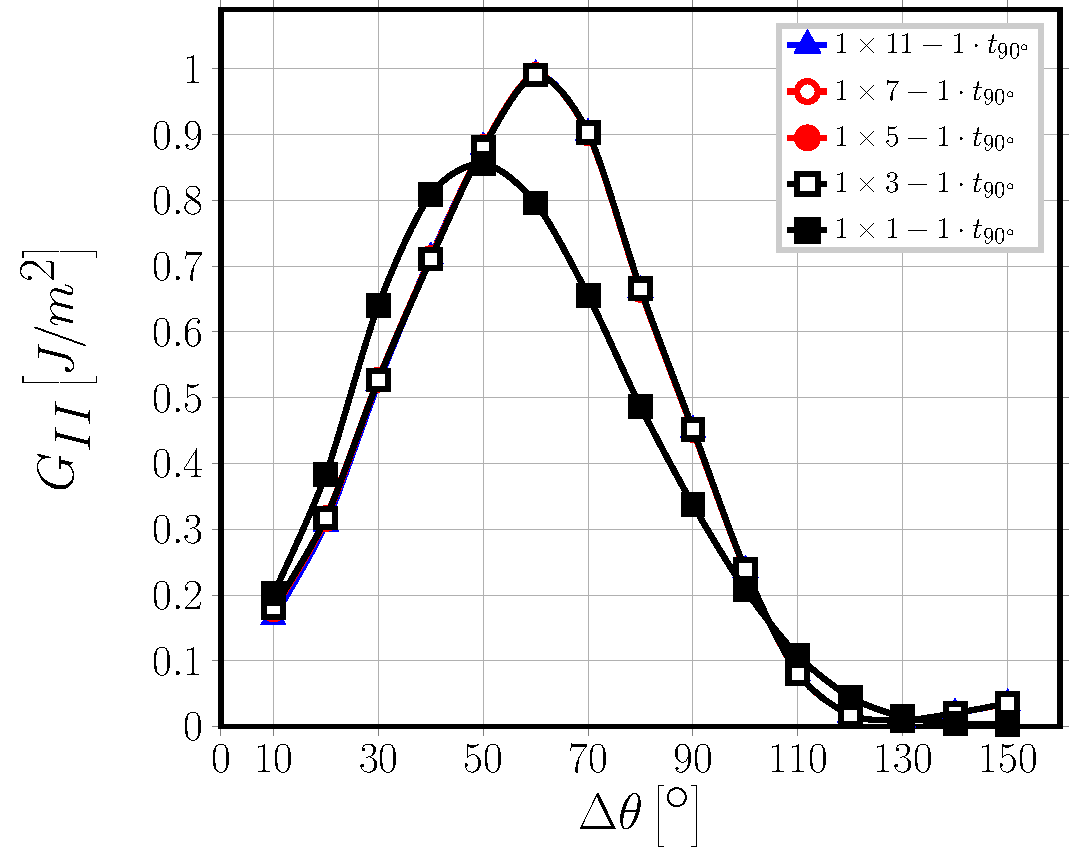
\includegraphics[height=0.375\textheight]{1xk-1-vf60-GII.pdf}
\caption{Effect of the presence of undamaged fiber rows in the $90^{\circ}$ layer on debond-$0^{\circ}/90^{\circ}$ interface interaction for Mode II ERR: models $1\times k-1\cdot t_{90^{\circ}}$. $V_{f}=60\%$, $\bar{\varepsilon}_{x}=1\%$.}\label{fig:1kGII}
\end{figure}

The results of Figures~\ref{fig:1kGI}, \ref{fig:1kGII}, \ref{fig:nkGI} and~\ref{fig:nkGII} imply that the mechanisms of debond-$0^{\circ}/90^{\circ}$ interface interaction described in Sec.~\ref{subsec:thickness} and Sec.~\ref{subsec:debonddebondinter} are actually very localized and that debond ERR is affected by the presence of the $0^{\circ}/90^{\circ}$ interface only when no fully bonded fiber is placed in between. Given that the number $k$ of fibers in the RUC vertical direction corresponds to the thickness of the $90^{\circ}$ ply measured in terms of number of fiber rows present through its thickness, the results presented here point to another conclusion: the ply-thickness effect does not seem to apply to debond growth, unless an \textit{ultra-thin} ply constituted by only one fiber row ($k=1$) is considered.\\

\begin{figure}[!htb]
\centering
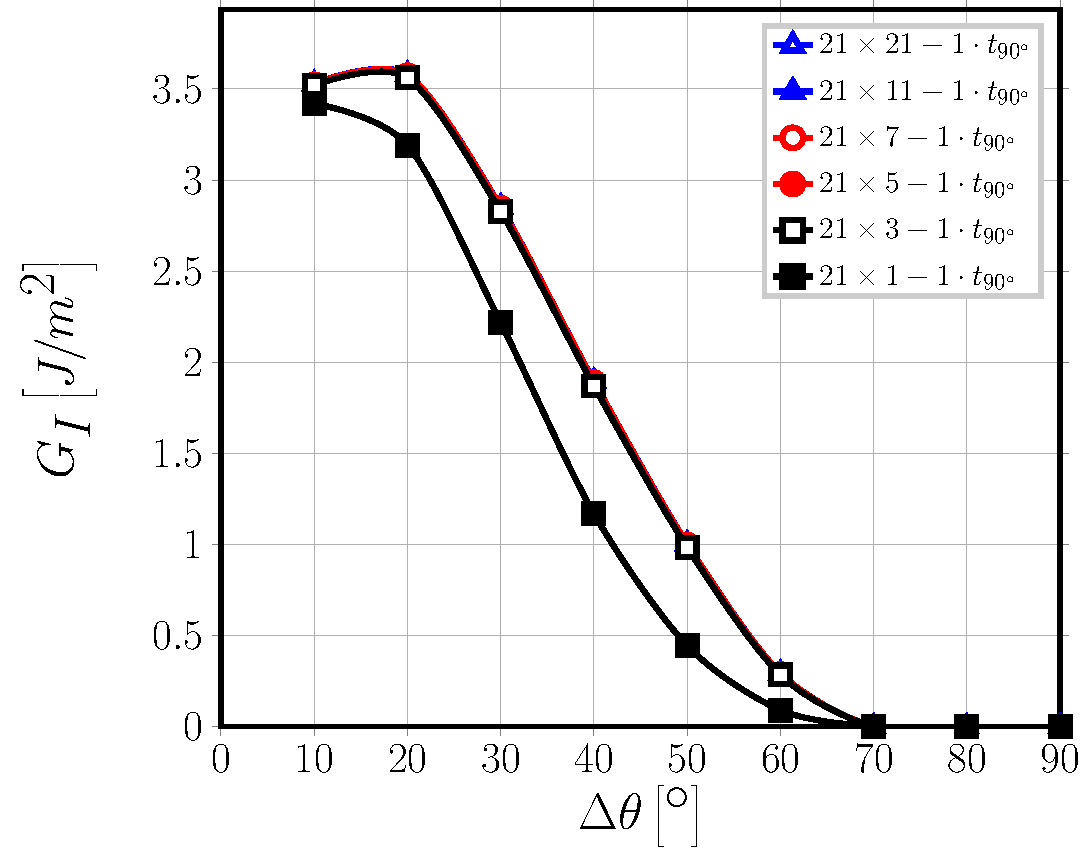
\includegraphics[height=0.375\textheight]{nxk-1-vf60-GI.pdf}
\caption{Effect of the presence of undamaged fiber rows in the $90^{\circ}$ layer on debond-$0^{\circ}/90^{\circ}$ interface interaction for Mode I ERR: models $n\times k-1\cdot t_{90^{\circ}}$. $V_{f}=60\%$, $\bar{\varepsilon}_{x}=1\%$.}\label{fig:nkGI}
\end{figure}

Analogous results can be found in~\cite{Velasco2018, Paris2018}, where the authors investigate the ply-thickness effect on debond growth in cross-ply laminates using: first, a single centrally-placed partially debonded fiber with surrounding matrix corresponding to $V_{f}=55\%$, embedded from all sides in a homogenized $90^{\circ}$ ply bounded by homogenized $0^{\circ}$ layers; second, one partially debonded fiber placed in the center and a second partially debonded fiber placed at an angle $\theta_{2}$ with respect to the horizontal direction with surrounding matrix corresponding to $V_{f}=55\%$, embedded from all sides in a homogenized $90^{\circ}$ ply bounded by homogenized $0^{\circ}$ layers. The thickness of the $0^{\circ}$ layer is chosen as reference and a $\left[0^{\circ}_{p},90^{\circ}_{r\cdot p}\right]_{S}$ laminate is considered. Carbon-epoxy and glass-epoxy systems are both studied. The thickness of the $90^{\circ}$ ply, $t_{90^{\circ}}=r\cdot t_{0^{\circ}}$, varies from $r=3$ (thick $90^{\circ}$ ply, $>100$ fiber diameters) to $r=0.1$ (thin $90^{\circ}$ ply, $\sim4-5$ fiber diameters). No measurable ply-thickness effect was observed. Experimental support to the claim that the ply-thickness effect has no influence on debond growth can be also found in the literature, in~\cite{Saito2012}. The authors conducted \emph{in-situ} observations of edge micro-cracks with an optical microscope on $\left[0^{\circ}_{2},90^{\circ}_{n},0^{\circ}_{2}\right]$ carbon fiber-epoxy laminates with $n=1,2,4$, corresponding to a $90^{\circ}$ ply thickness of respectively $40\ [\mu m]$ ($\sim 6-8$ fiber diameters), $80\ [\mu m]$  ($\sim 12-16$ fiber diameters) and $160\ [\mu m]$  ($\sim 24-32$ fiber diameters). For $n=1$, i.e. the case of a very thin $90^{\circ}$ ply, isolated debonds appear at a lower value of the applied strain than in thicker plies (at $0.4\%$ vs $0.7\%$) while growth and coalescence of debonds is suppressed and no transverse crack can be observed even at a strain of $1.5\%$. The ply-thickness effect was thus observed in~\cite{Saito2012} for transverse cracks, i.e. coalescence of debonds was delayed to higher strains and even suppressed, but not for debond growth. The analysis presented in this article brings new arguments to the claim that the ply-thickness effect does not influence the growth of debonds. 

\begin{figure}[!htb]
\centering
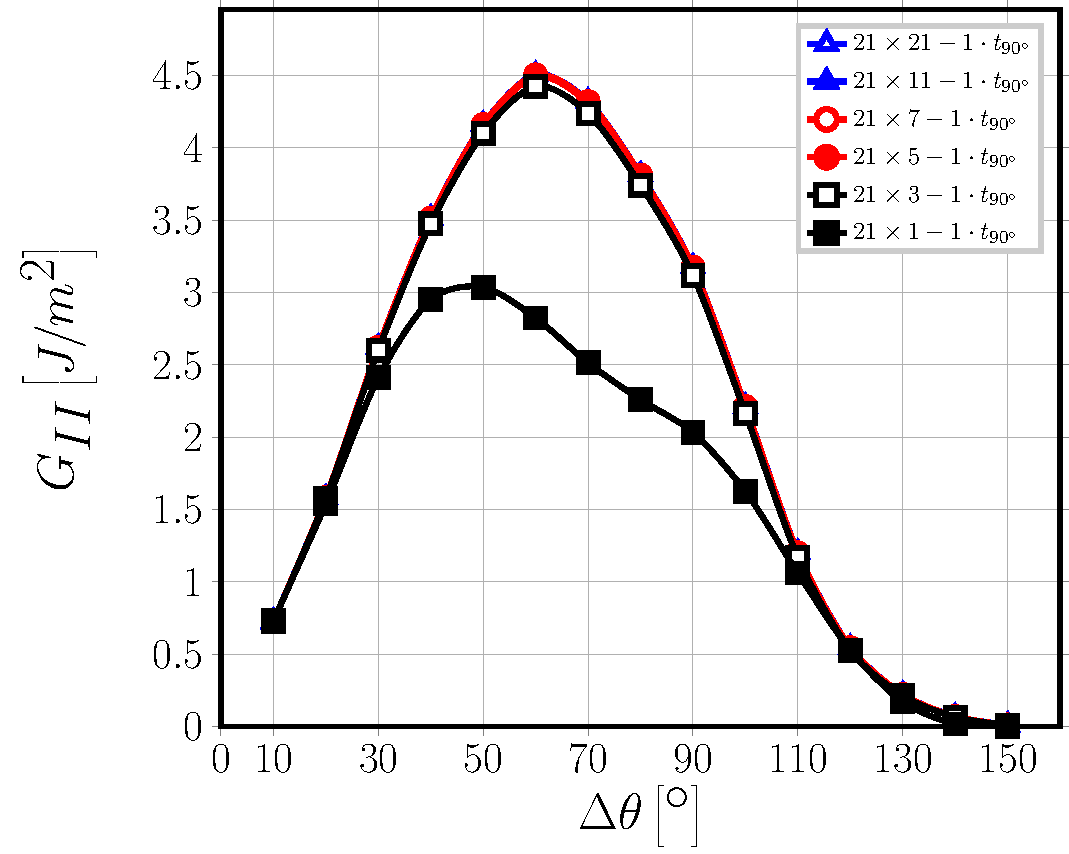
\includegraphics[height=0.375\textheight]{nxk-1-vf60-GII.pdf}
\caption{Effect of the presence of undamaged fiber rows in the $90^{\circ}$ layer on debond-$0^{\circ}/90^{\circ}$ interface interaction for Mode II ERR: models $n\times k-1\cdot t_{90^{\circ}}$. $V_{f}=60\%$, $\bar{\varepsilon}_{x}=1\%$.}\label{fig:nkGII}
\end{figure}

%%%%%%%%%%%%%%%%%%%%%%%%%%%%%%%%%%%%%%%%%%%%%%%%%%%%%%%%%%%%%%%%%%%
% 4. CONCLUSIONS AND OUTLOOK
%%%%%%%%%%%%%%%%%%%%%%%%%%%%%%%%%%%%%%%%%%%%%%%%%%%%%%%%%%%%%%%%%%%

\section{Conclusions}

Different models of Repeating Unit Cell, representing different cross-ply laminates, have been studied in order to investigate the effect of the presence of the $0^{\circ}$ layer and of its thickness on debond Energy Release Rate for interactive and non-interactive debonds. A particular damage state is studied, in which only the central row of fibers of the $90^{\circ}$ ply possesses debonds. The thickness of the $90^{\circ}$ ply is measured in terms of the number of fiber rows in the layer; the $0^{\circ}$ layer is on the other hand modelled as a homogenized material, the thickness of which is a multiple of the $90^{\circ}$ ply thickness. In order to investigate the mechanisms of the debond-$0^{\circ}/90^{\circ}$ interface interaction, Mode I and Mode II ERR of cross-ply RUCs are compared with those of RUCs with equivalent boundary conditions on the upper boundary: free surface; coupling conditions on the vertical displacements; an applied linear distribution of the horizontal displacement; coupling conditions on the vertical displacements superimposed to an applied linear distribution of the horizontal displacement (this last combination represents the most extreme effect of the $0^{\circ}$ layer on debond growth). It has been found that:
\begin{itemize}
\item by forcing the $0^{\circ}/90^{\circ}$ interface to remain approximately straight and controlling the uniformity of the horizontal displacements in the composite (and thus in the $90^{\circ}$ ply), the presence of the $0^{\circ}$ layer causes more homogeneous local (i.e. in the debond neighborhood) strains, reducing the ERR at the debond crack tip;
\item when increasing the thickness of the $0^{\circ}$ layer, the effect of the presence of the $0^{\circ}$ layer on debond ERR remains the same as in the case $t_{0^{\circ}}=t_{90^{\circ}}$;
%\item no difference in ERR is seen when one or more rows of fibers with no damage are present between the debond and the $0^{\circ}/90^{\circ}$ interface, a change is observed only no row of undamaged fibers is present between the debond and the $0^{\circ}/90^{\circ}$ interface;
\item no effect of the $90^{\circ}$ layer thickness, measured in terms of number of fiber rows, is observed; a reduction in ERR takes place only when the thickness is reduced to only one fiber row.
\end{itemize}
The results reported in this article strengthen the claim that the ply-thickness effect does not influence the growth of individual debonds, as previously suggested in the literature~\cite{Saito2012,Herraez2015,Velasco2018, Paris2018}. 

%%%%%%%%%%%%%%%%%%%%%%%%%%%%%%%%%%%%%%%%%%%%%%%%%%%%%%%%%%%%%%%%%%%
% ACKNOWLEDGEMENTS
%%%%%%%%%%%%%%%%%%%%%%%%%%%%%%%%%%%%%%%%%%%%%%%%%%%%%%%%%%%%%%%%%%%

\begin{acks}
Luca Di Stasio gratefully acknowledges the support of the European School of Materials (EUSMAT) through the DocMASE Doctoral Programme and the European Commission through the Erasmus Mundus Programme.
\end{acks}

\bibliographystyle{SageV}
\bibliography{refs}

\end{document}
